
\documentclass[aspectratio=169,11pt]{beamer}

% Theme
\usetheme{Madrid}

% Packages
\usepackage{graphicx}
\usepackage{booktabs}
\usepackage{xcolor}

% Presentation information
\title{Exoplanets Through Data}
\subtitle{Exploring the Diversity of Planetary Systems}
\author{Margarida Castro Neves}
%\date{\monthname[\month] \the\year}

\begin{document}
	% Title slide
	{ 
		% Background image
		\usebackgroundtemplate{
		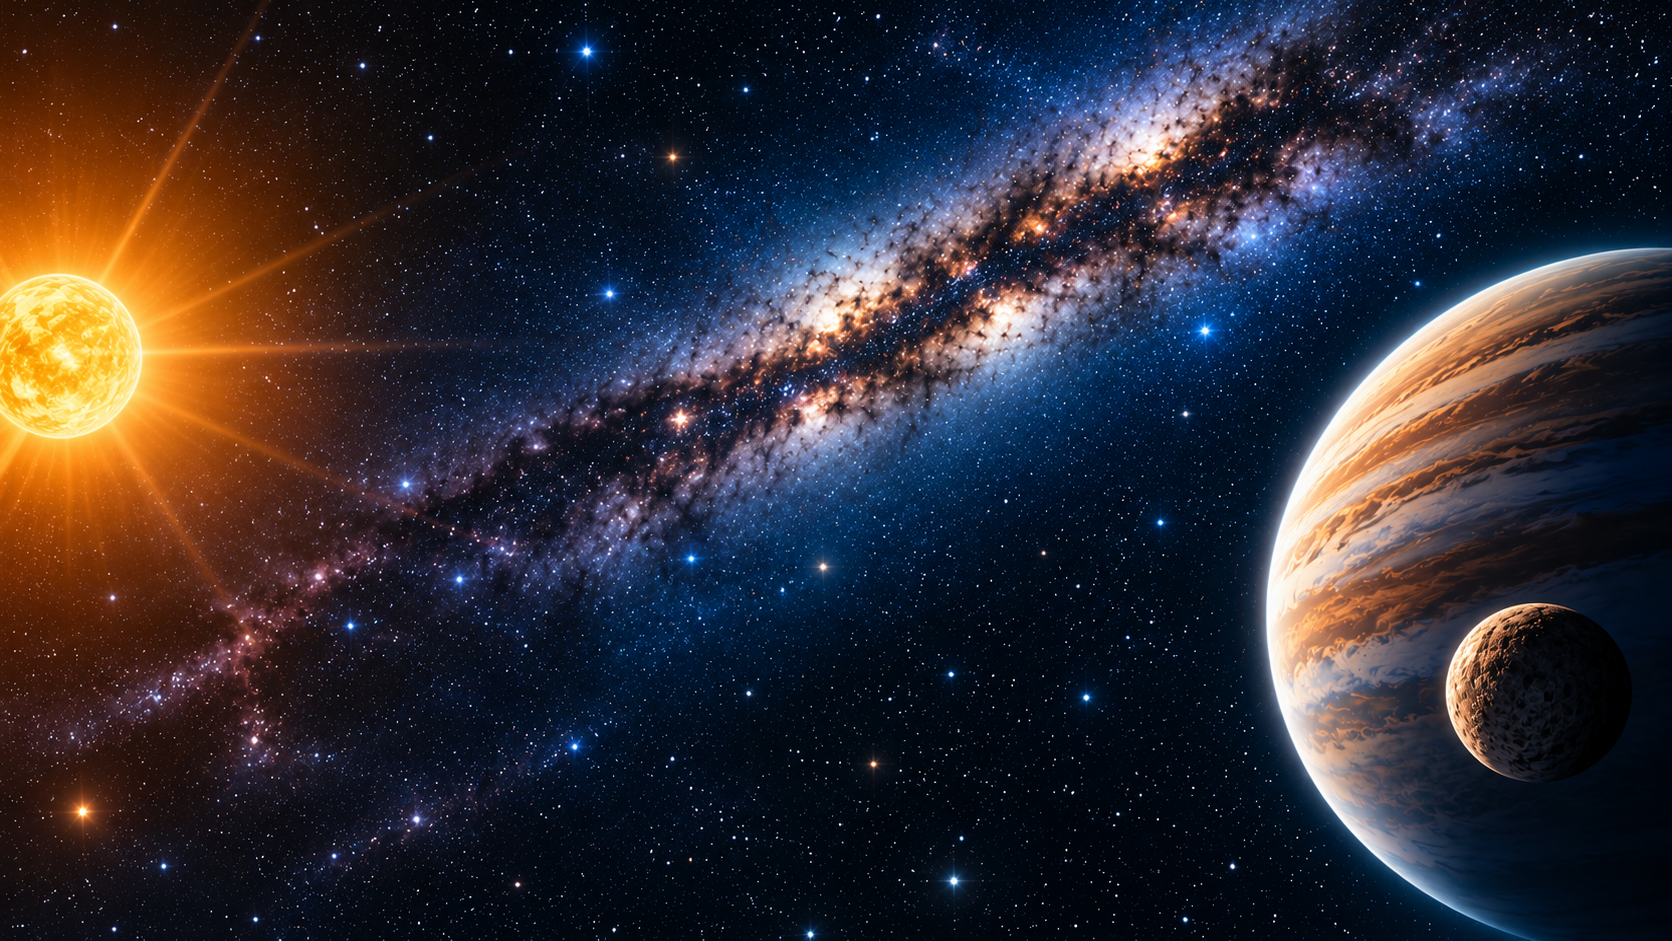
\includegraphics[width=\paperwidth,height=\paperheight]
		{figures/exoplanets.png}
		}

	% Title slide
	\begin{frame}[plain]
	
		\vspace{3cm}

		\begin{center}
		{\Huge\bfseries\color{white}
		Exoplanets Through Data}

		\vspace{0.5cm}

		{\large\color{white}
		Exploring the Diversity of Planetary Systems}
		\end{center}
		
		\vspace{2cm}
		
		 {\large\color{white}
			Margarida Castro Neves}
		

	\end{frame}
	}
	% Slide 1: Introduction
	
	\begin{frame}{Introduction: What Are Exoplanets?}
	
	\begin{columns}[T,onlytextwidth]
	
	% Left column: Definition and motivation
	\begin{column}{0.8\textwidth}
	
	\textbf{Exoplanets}
	
	\begin{itemize}
	\item Planets orbiting stars outside our Solar System.
	\item They exhibit a remarkable diversity in size, mass,
	composition, and orbital characteristics.
	\end{itemize}
	
	\vspace{0.3cm}
	
	\textbf{Why study them?}
	
	\begin{itemize}
	\item Understand how planetary systems form and evolve.
	\item Explore the diversity of planets beyond our
	Solar System.
	\item Investigate the conditions that could support life.
	\end{itemize}
	
	\end{column}
	
	% Right column: Image
	\begin{column}{0.42\textwidth}
%	\centering
%	\includegraphics[width=\textwidth]
%	{figures/exoplanet\_types.png}
	
%	\vspace{0.2cm}
%	{\scriptsize Artist's illustration of different types
%	of exoplanets.}
	\end{column}
	
	\end{columns}
	
	\vfill
	
	\begin{block}{Research Objective}
	What can the statistical analysis of known exoplanets
	tell us about their discovery, physical properties,
	and planetary systems?
	\end{block}
	
	\end{frame}

% Slide 2: Dataset and Methodology

	\begin{frame}{Dataset and Methodology}
	
	\begin{block}{Data Source}
		\textbf{NASA Exoplanet Archive}: \href{https://exoplanetarchive.ipac.caltech.edu/}{https://exoplanetarchive.ipac.caltech.edu/}
		
		\begin{itemize}
			\item Table: \texttt{PSCompPars}: confirmed exoplanets and their physical
			and orbital parameters
			
			\item Provides a consolidated set of planetary parameters.
		\end{itemize}
	\end{block}
	
	\vspace{0.2cm}
	
	\begin{block}{Data Retrieval}
		\begin{itemize}
			\item Data accessed through the
			\textbf{Table Access Protocol (TAP)}.
			\item Queries executed in Python using
			\textbf{PyVO}, data converted into a Pandas DataFrame.
			
		\end{itemize}
	\end{block}
	
	\vspace{0.2cm}
	
	% Main parameters investigated
	\textbf{Main parameters investigated}

	\vspace{0.1cm}

	\begin{columns}[T,onlytextwidth]
	
		\begin{column}{0.32\textwidth}
			\begin{itemize}
				\setlength{\itemsep}{2pt}
				\item Discovery year
				\item Discovery method
			\end{itemize}
		\end{column}
	
		\begin{column}{0.32\textwidth}
			\begin{itemize}
			\setlength{\itemsep}{2pt}
			\item Planet radius and mass
			\item Orbital period
			\end{itemize}
		\end{column}
	
		\begin{column}{0.32\textwidth}
			\begin{itemize}
			\setlength{\itemsep}{2pt}
			\item Host star
			\item Planet count per system
			\end{itemize}
		\end{column}
	\end{columns}
	
	\end{frame}
	
	% Slide 3: History of Exoplanet Discoveries

\begin{frame}{History of Exoplanet Discoveries}
	
	\begin{columns}[T,onlytextwidth]
		
		% Left column: Main observations
		\begin{column}{0.25\textwidth}
			
			\textbf{A growing population}
			
			\begin{itemize}
				
				\item Observational techniques over time,
				space missions
				
			\end{itemize}
			
			\vspace{0.1cm}
			
			\textbf{Notable peaks}
			
			\begin{itemize}
				\item 2014, 2016: validation of Kepler planets.
			\end{itemize}
			\begin{block}{Key Observation}
				More discoveries reflect better technology and validation methods.
			\end{block}
			
		\end{column}
		% Right column: Discovery plot
		\begin{column}{0.76\textwidth}
			\centering
			
			{\large\bfseries Exoplanet Discoveries per Year}
			
			\vspace{0.2cm}
			
			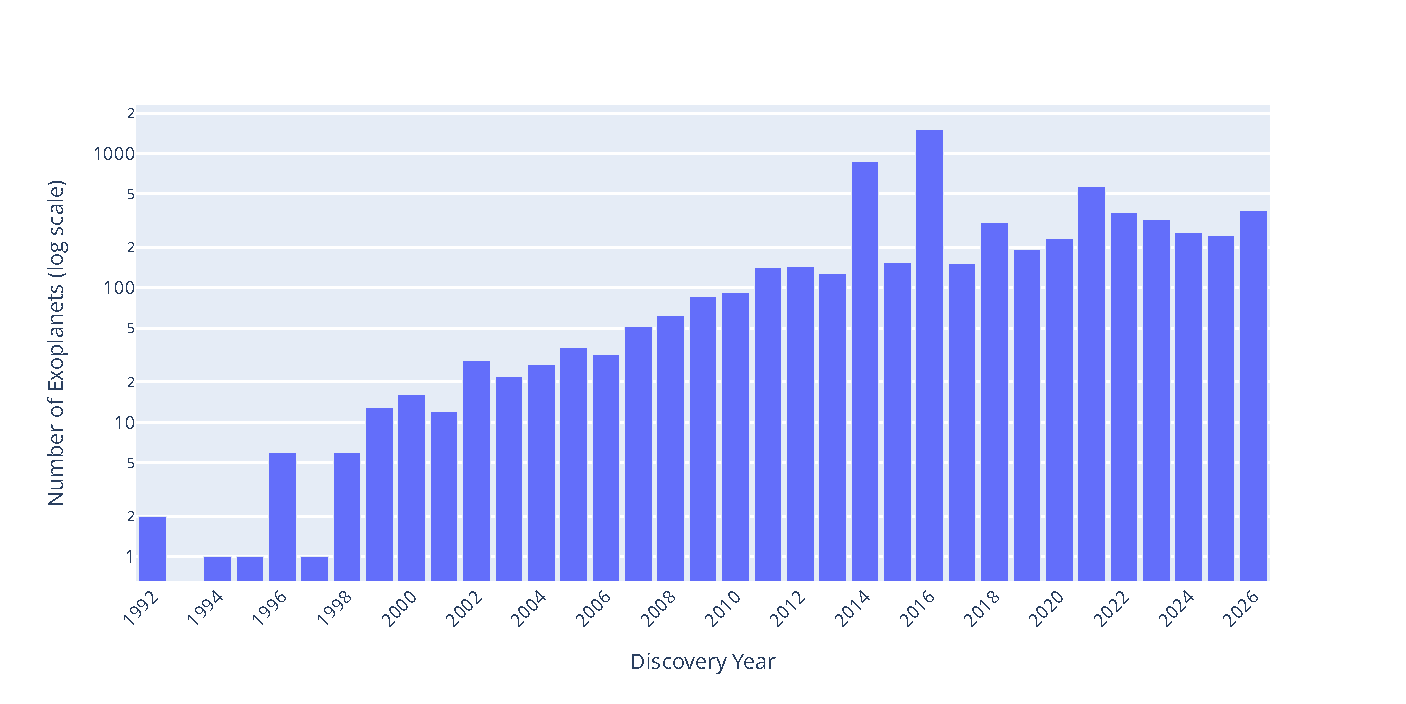
\includegraphics[width=\textwidth]
			{figures/discoveries_per_year.pdf}
			
		\end{column}
		
		% Right column: Discovery plot

	\end{columns}
	
	\vfill
	
\end{frame}
% Slide 4: Exoplanet Discovery Methods

\begin{frame}{How Are Exoplanets Discovered? The 3 Main Methods}
	
	\begin{columns}[T,onlytextwidth]
		
		% Transit method
		\begin{column}{0.32\textwidth}
			\centering
			\textbf{Transit Method}
			
			\vspace{0.2cm}
			
			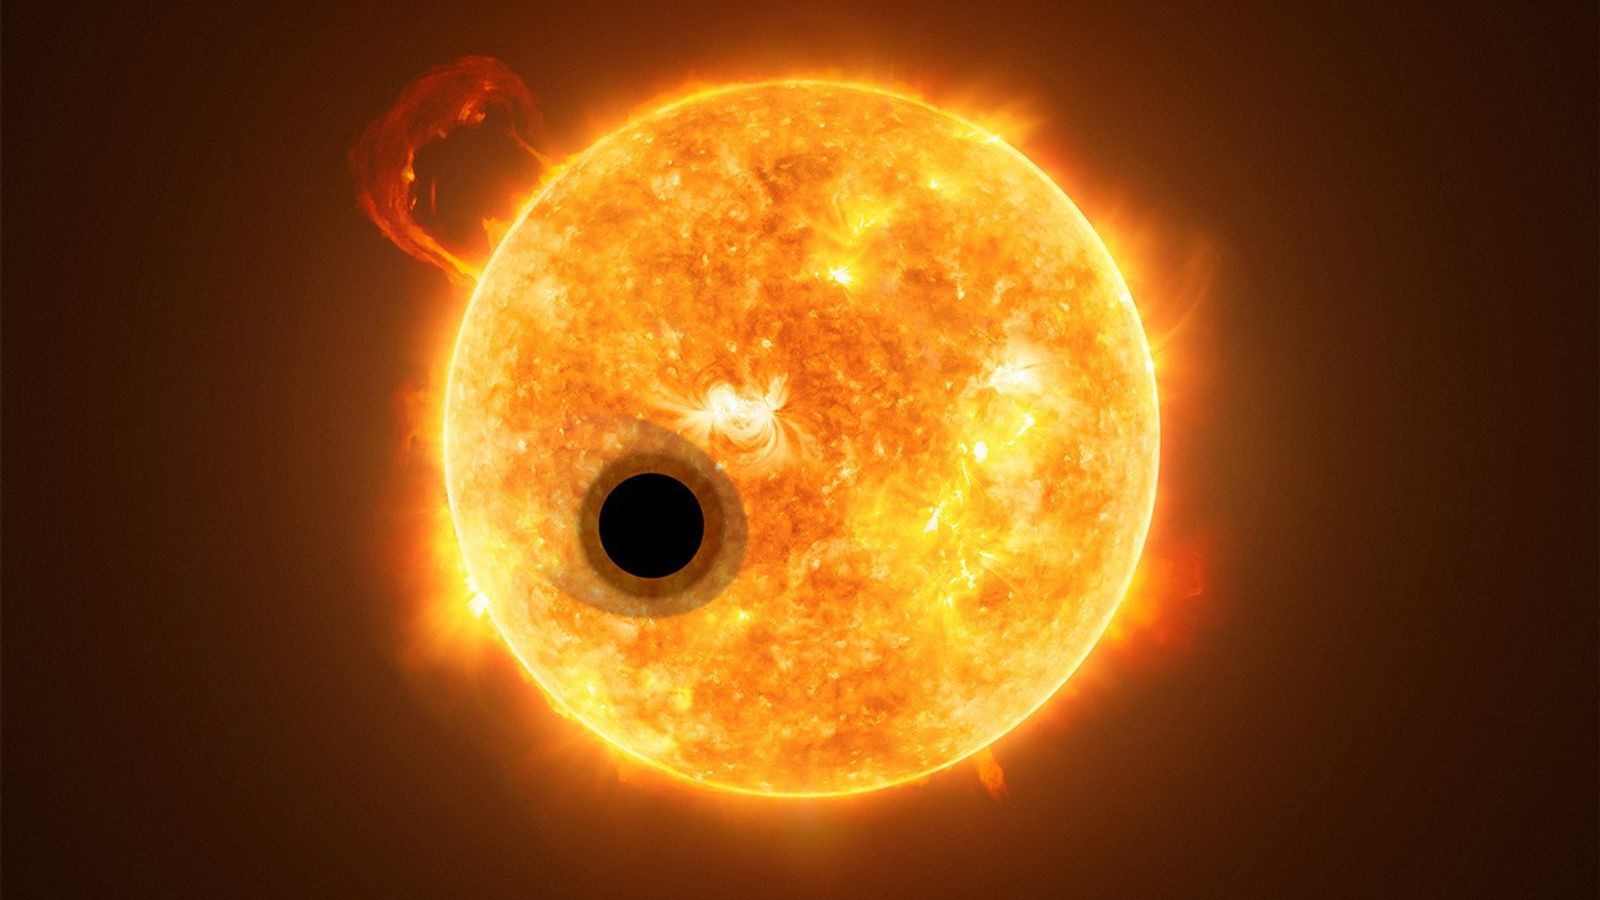
\includegraphics[
			width=\textwidth,
			height=3cm,
			keepaspectratio
			]
			{figures/Wasp-107b.jpeg}
			
			\vspace{0.15cm}
			
			\small
			Detects the decrease in stellar brightness when a planet
			passes in front of its host star.
		\end{column}
		
		% Radial velocity
		\begin{column}{0.32\textwidth}
			\centering
			\textbf{Radial Velocity}
			
			\vspace{0.2cm}
			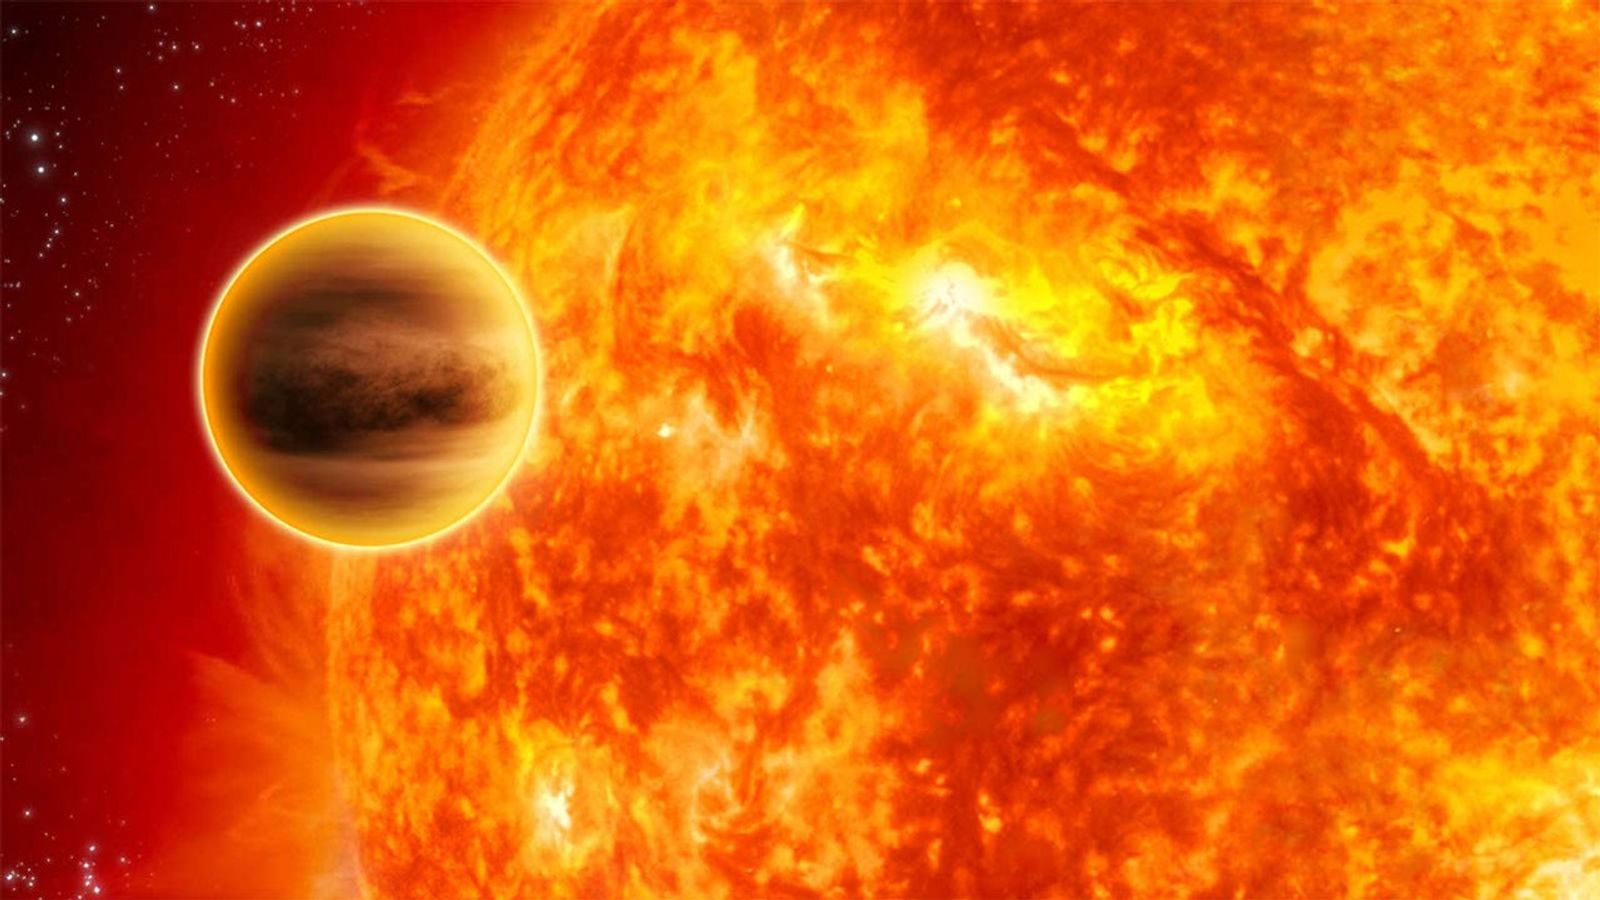
\includegraphics[
			width=\textwidth,
			height=3cm,
			keepaspectratio
			]
			{figures/artists_concept_of_51_Pegasi_b.jpeg}
			
			\vspace{0.15cm}
			
			\small
			Measures the motion of a star caused by the gravitational
			pull of an orbiting planet.
		\end{column}
		
		% Microlensing
		\begin{column}{0.32\textwidth}
			\centering
			\textbf{Microlensing}
			
			\vspace{0.2cm}
			
			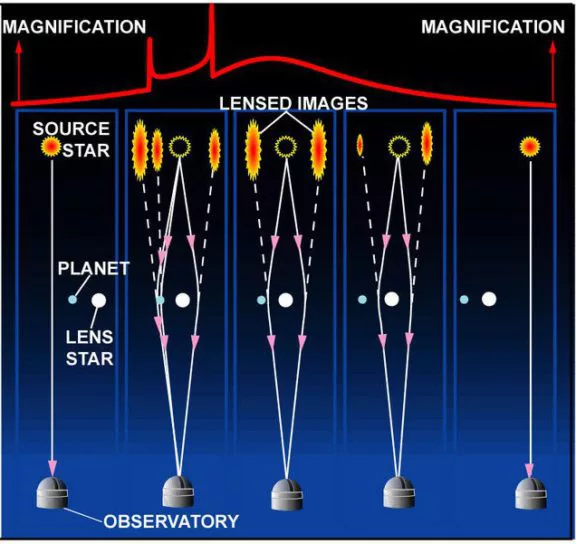
\includegraphics[
			width=\textwidth,
			height=3cm,
			keepaspectratio
			]
			{figures/microlensing3.png}
			
			\vspace{0.15cm}
			
			\small
			Detects the temporary brightening of a background star
			due to gravitational lensing.
		\end{column}
		
	\end{columns}
	
	{\tiny
		Images: \href{https://science.nasa.gov/exoplanets/how-we-find-and-characterize/}{NASA},
		\href{https://www.planetary.org/articles/space-warping-planets-the-microlensing-method/}{The Planetary Society}
	}
	\vspace{0.15cm}
	
	\begin{block}{Discovery Statistics}
		\centering
		Transit, radial velocity and microlensing account for
		the three leading discovery methods in the analysed dataset.
	\end{block}
	\vfill

	\end{frame}

% Slide 5: Discovery Statistics

\begin{frame}{Which Methods Discover the Most Exoplanets?}
	
	\begin{columns}[T,onlytextwidth]
		
		% Left: Discovery counts
		\begin{column}{0.48\textwidth}
			
			\textbf{All discovery methods}
			
			\vspace{0.3cm}
			
			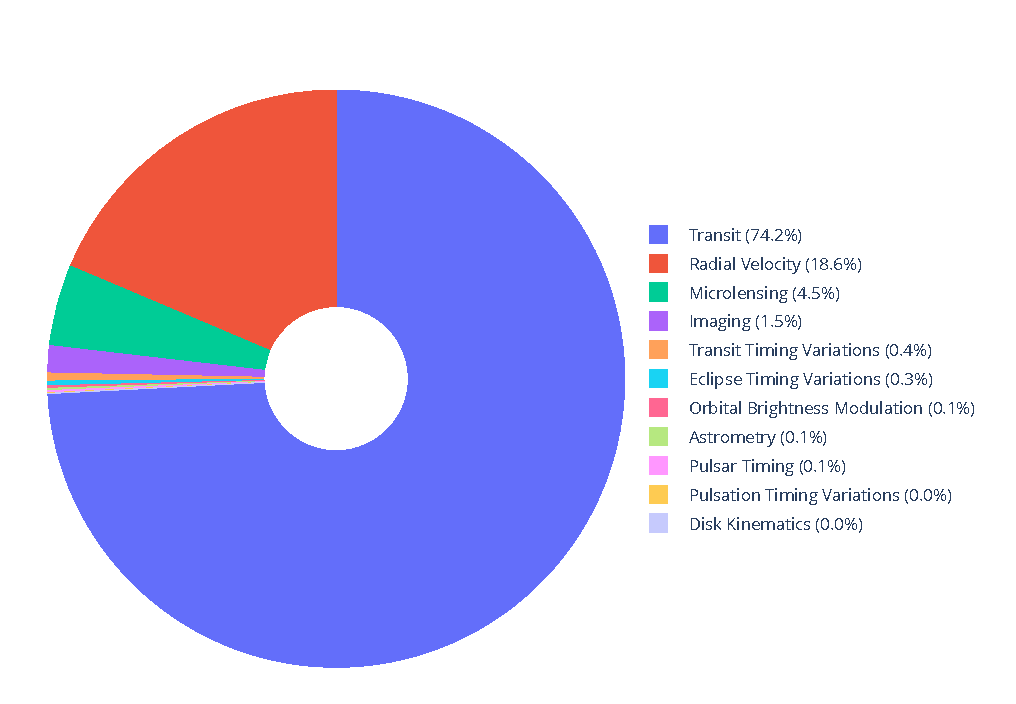
\includegraphics[width=\textwidth]
			{figures/discoveries_per_method.pdf}
			
			{\tiny Number of confirmed planets by discovery method.}
			
		\end{column}
		
		% Right: Main observations
		\begin{column}{0.48\textwidth}
			
			\textbf{Key observations}
			
			\begin{itemize}
				\setlength{\itemsep}{8pt}
				
				\item Transit is the dominant discovery method
				in the dataset.
				
				\item Radial velocity is another major contributor
				to the confirmed exoplanet population.
				
				\item Microlensing accounts for a smaller,
				but scientifically important, fraction.
			\end{itemize}
			
			\vspace{0.3cm}
			
			\textbf{Next question}
			
			Do different discovery methods detect planets
			with different physical properties?
			
		\end{column}
		
	\end{columns}
	
\end{frame}

% Slide 6: Planetary Properties by Discovery Method
\begin{frame}{Planetary Properties by Discovery Method}
	
	\begin{columns}[T,onlytextwidth]
		
		\begin{column}{0.65\textwidth}
			\centering
			\textbf{Radius and Mass by Discovery Methods}
			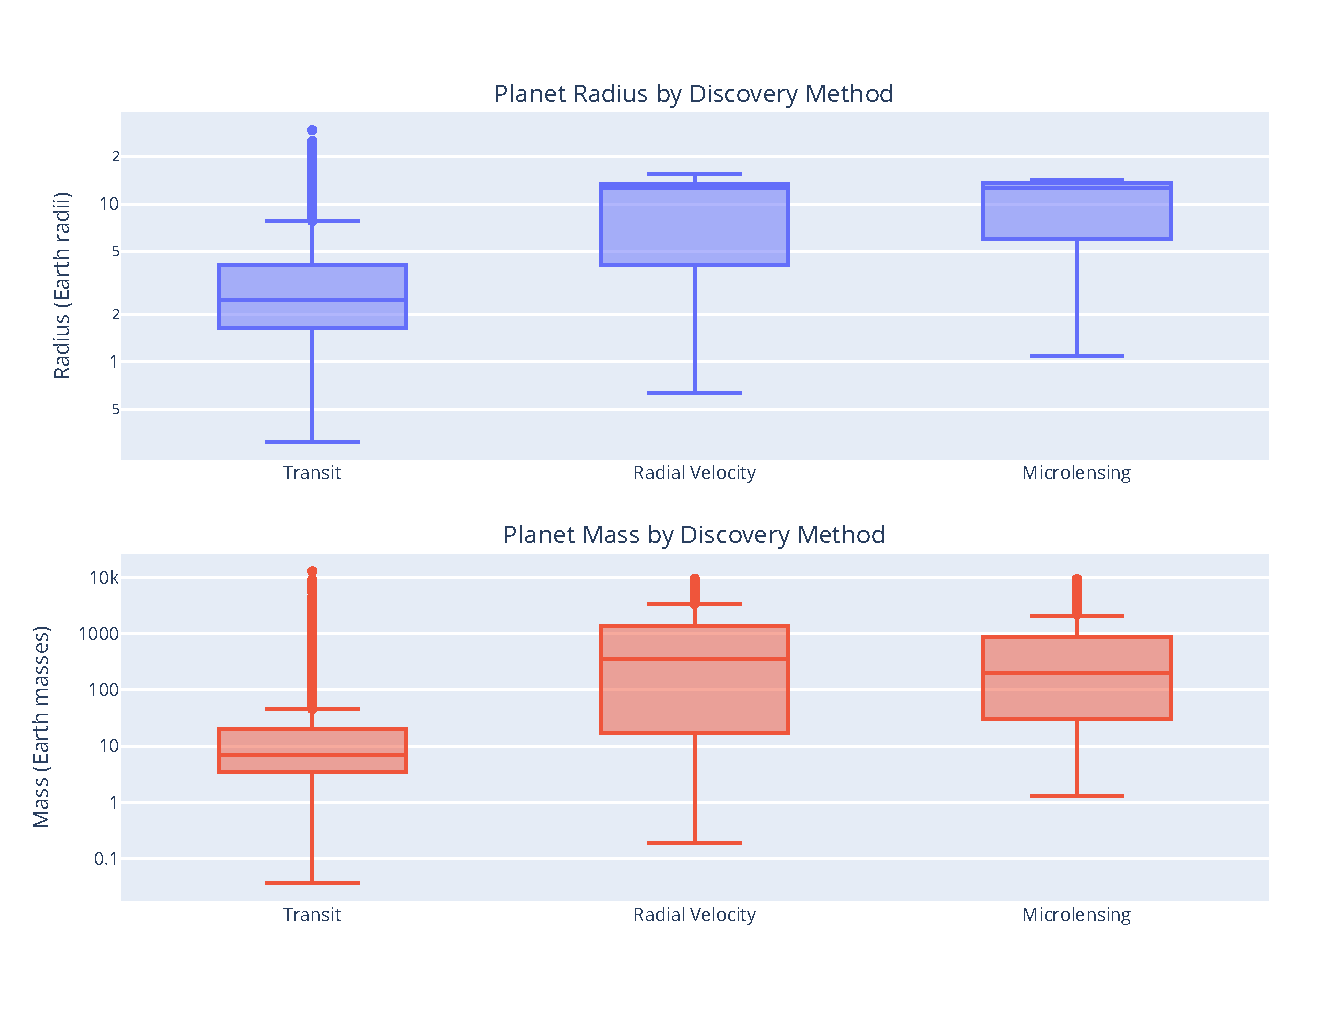
\includegraphics[width=\textwidth]
			{figures/radius_and_mass_by_method.pdf}
		\end{column}
		
		\begin{column}{0.32\textwidth}
			\textbf{Key Observations}
			
			\begin{itemize}
				\setlength{\itemsep}{8pt}
				\item Planet properties vary across discovery methods.
				\item Transit shows lower median values.
				\item Radial velocity and microlensing show higher medians.
			\end{itemize}
			\begin{block}{Caution}
				Differences reflect observational selection effects.
			\end{block}
			
		\end{column}
		
	\end{columns}
	
	\vfill
	
	\begin{block}{Important Consideration}
		Differences between methods are influenced by their
		detection sensitivities and observational selection effects.
	\end{block}
	
\end{frame}

% Slide 7: Relationship Between Planet Mass and Radius
\begin{frame}{Relationship Between Planet Mass and Radius}
	
	\begin{columns}[T,onlytextwidth]
		
		\begin{column}{0.65\textwidth}
			\centering
			
			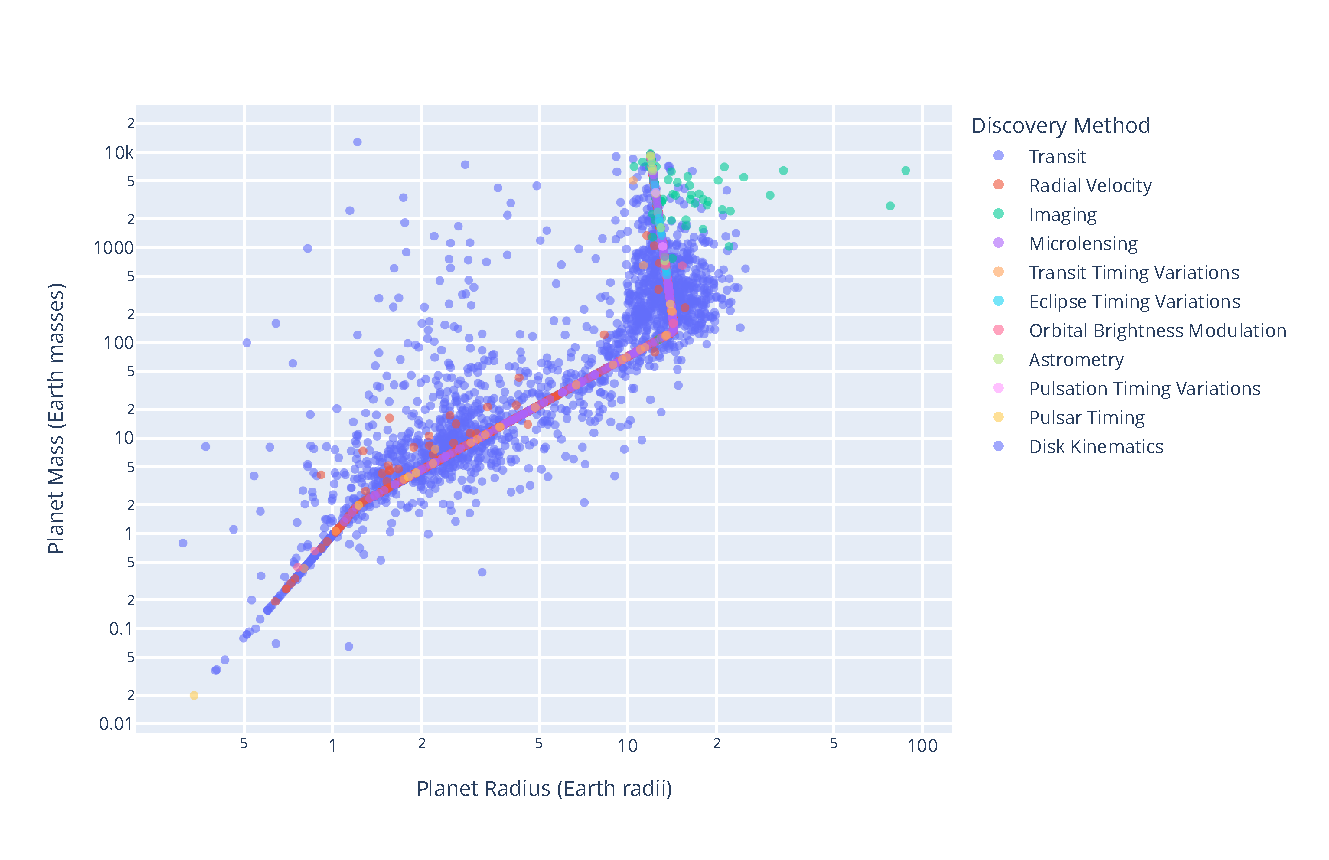
\includegraphics[
			width=\textwidth,
			height=0.65\textheight,
			keepaspectratio
			]{figures/mass_vs_radius.pdf}
		\end{column}
		
		\begin{column}{0.32\textwidth}
			\textbf{Key Observations}
			
			\begin{itemize}
				\setlength{\itemsep}{8pt}
				\item Planet mass strongly increases with planetary radius..
				\item The relationship shows some variation across planets.
				\item Planet composition  contributes to differences in density.
			\end{itemize}
		\end{column}
		
	\end{columns}
	
	\vfill
\end{frame}
	\begin{frame}{When Data Processing Shapes the Results}
		\begin{columns}[T,onlytextwidth]
			\begin{column}{0.58\textwidth}
				\centering
				\textbf{Removing Transit and Imaging methods:}
				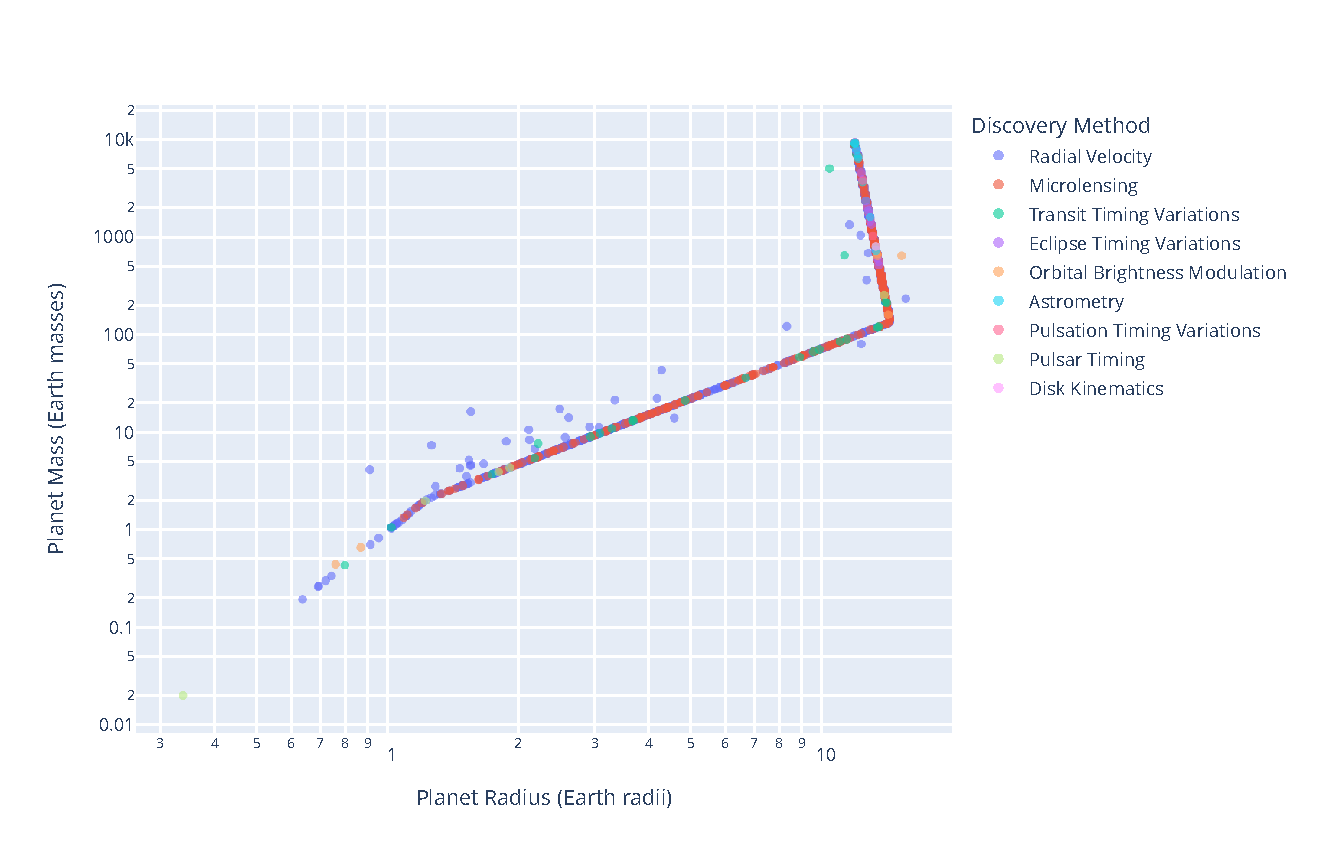
\includegraphics[
				width=\textwidth,
				height=0.65\textheight,
				keepaspectratio
				]{figures/mass_vs_radius_filtered.pdf}
			\end{column}
			
			\begin{column}{0.38\textwidth}
				\textbf{Why the L-shaped pattern?}
				\begin{itemize}
					\setlength{\itemsep}{7pt}
					\item Some planetary radii are calculated,
					not directly measured.
					\item The Archive uses the Chen \& Kipping
					(2017) mass--radius relation.
					\item For giant planets, the relation predicts
					nearly constant radii over a wide
					mass range.
				\end{itemize}
			\end{column}
		\end{columns}
	
		\begin{block}{Key Lesson}
			Understanding how data are generated is essential
			for interpreting statistical patterns.
		\end{block}
		
	\end{frame}
%\begin{frame}{Comparing Published and Composite Parameters}
%	\begin{columns}[T,onlytextwidth]
%		\begin{column}{0.55\textwidth}
%			\textbf{Two Archive Tables}
%			\begin{itemize}
%				\item \texttt{PS}: Individual published parameter records.
%				\item \texttt{PSCompPars}: Consolidated planetary parameters.
%			\end{itemize}
%			
%			\vspace{0.2cm}
%			\textbf{Key Observations}
%			\begin{itemize}
%				\item Fewer planets have both mass and radius in \texttt{PS}.
%				\item Some methods is absent from the filtered sample.
%				\item Data availability affects the observed patterns.		
%			\end{itemize}
%		\end{column}
%		
%		\begin{column}{0.45\textwidth}
%			\centering
%			\includegraphics[width=\textwidth]
%			{figures/mass_radius_ps.pdf}
%			{\scriptsize Mass--radius relation using published parameters.}
%		\end{column}
%	\end{columns}
%	
%	\vfill
%	\begin{block}{Key Takeaway}
%		The choice of data source and available measurements
%		can influence the statistical patterns we observe.
%	\end{block}
%\end{frame}

\begin{frame}{Conclusions and Limitations}
	
	\textbf{Main Findings}
	\begin{itemize}
		\item Exoplanet discoveries have increased substantially
		over the past decades.
		\item The transit method dominates the confirmed
		exoplanet sample.
		\item Planet mass and radius show a strong positive
		correlation ($\rho = 0.93$).
		\item Discovery methods reveal different distributions
		of planetary properties.
	\end{itemize}
	
	\vspace{0.3cm}
	
	\textbf{Limitations}
	\begin{itemize}
		\item Missing measurements limit some analyses.
		\item Detection methods introduce observational
		selection effects.
		\item Some planetary radii are calculated rather
		than directly measured.
	\end{itemize}
	
	\vfill
	
	\begin{block}{Final Takeaway}
		Exoplanet data reveal remarkable planetary diversity,
		but statistical patterns must be interpreted in the
		context of observational and data-processing biases.
	\end{block}
	
\end{frame}

\end{document}